\section{Binomial Probability}
In this section you will learn to:
\begin{enumerate}
    \item Recognize when to use the binomial probability distribution
    \item Derive the formula for the binomial probability distribution
    \item Calculate probabilities for a binomial probability experiment
\end{enumerate}

In this section, we consider problems that involve a sequence of trials, where each trial has only two outcomes, a \textbf{success} or a \textbf{failure}. These trials are independent, that is, the outcome of one does not affect the outcome of any other trial. The probability of success, \( p \), and the probability of failure, \( 1 - p \), remains the same throughout the experiment. These problems are called \textbf{binomial probability problems}. Since these problems were researched by Swiss mathematician Jacques Bernoulli around 1700, they are also called \textbf{Bernoulli trials}.

We give the following definition:

\begin{summarybox}{Binomial Experiment}

    A binomial experiment satisfies the following four conditions:
    \begin{itemize}
        \item There are only two outcomes, a success or a failure, for each trial.
        \item The same experiment is repeated several times.
        \item The trials are independent; that is, the outcome of a particular trial does not affect the outcome of any other trial.
        \item The probability of success remains the same for every trial.
    \end{itemize}
\end{summarybox}

This probability model will give us the tools to solve many real-life problems, such as:
\begin{itemize}
    \item If a coin is flipped 10 times, what is the probability that it will fall heads 3 times?
    \item If a basketball player makes 3 out of every 4 free throws, what is the probability that he will make 7 out of 10 free throws in a game?
    \item If a medicine cures 80\% of the people who take it, what is the probability that among the ten people who take the medicine, 6 will be cured?
    \item If a microchip manufacturer claims that only 4\% of his chips are defective, what is the probability that among the 60 chips chosen, exactly three are defective?
    \item If a telemarketing executive has determined that 15\% of the people contacted will purchase the product, what is the probability that among the 12 people who are contacted, 2 will buy the product?
\end{itemize}

We now consider the following example to develop a formula for finding the probability of $k$ successes in $n$ Bernoulli trials.

\begin{example}
    A baseball player has a batting average of .300. If he bats four times in a game, find the probability that he will have
    \begin{enumerate}
        \item 4 hits
        \item 3 hits
        \item 2 hits
        \item 1 hit
        \item no hits.
    \end{enumerate}
\end{example}

\begin{solution}
    Let \( S \) denote that the player gets a hit, and \( F \) denote that he does not get a hit. This is a binomial experiment because it meets all four conditions. First, there are only two outcomes, \( S \) or \( F \). Clearly the experiment is repeated four times. Lastly, if we assume that the player's skillfulness to get a hit does not change each time he comes to bat, the trials are independent with a probability of .3 of getting a hit during each trial.

    We draw a tree diagram to show all situations. See figure \ref{figure_bernoulli_tree}.
    \begin{figure}[ht!]
        \label{figure_bernoulli_tree}
        \caption[short]{Tree Diagram for 4 Bernoulli trials}
        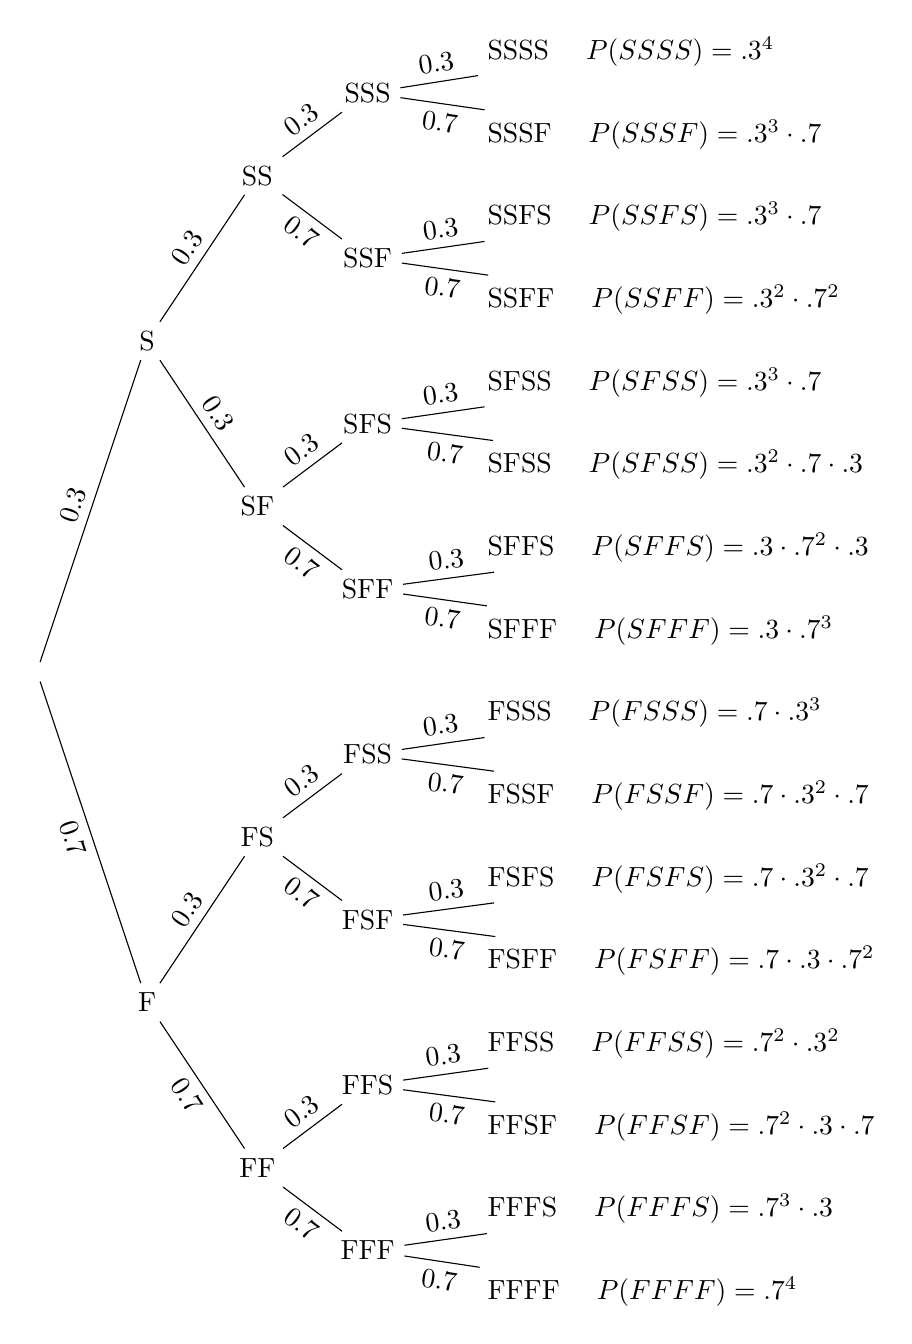
\begin{tikzpicture}[grow=right, sloped, scale= .7]
            \tikzstyle{level 1}=[level distance=2cm, sibling distance=12cm]
            \tikzstyle{level 2}=[level distance=2cm, sibling distance=6cm]
            \tikzstyle{level 3}=[level distance=2cm, sibling distance=3cm]
            \tikzstyle{level 4}=[level distance=2cm, sibling distance=1.5cm]
            \node {}
            child {
                    node {F}
                    child {
                            node {FF}
                            child {
                                    node {FFF}
                                    child {
                                            node[right] {FFFF \quad $P(FFFF) = .7^4$}
                                            edge from parent
                                            node[below] {0.7}
                                        }
                                    child {
                                            node[right] {FFFS \quad $P(FFFS) = .7^3 \cdot .3$}
                                            edge from parent
                                            node[above] {0.3}
                                        }
                                    edge from parent
                                    node[below] {0.7}
                                }
                            child {
                                    node {FFS}
                                    child {
                                            node[right] {FFSF \quad $P(FFSF) = .7^2 \cdot .3 \cdot .7$}
                                            edge from parent
                                            node[below] {0.7}
                                        }
                                    child {
                                            node[right] {FFSS \quad $P(FFSS) = .7^2 \cdot .3^2$}
                                            edge from parent
                                            node[above] {0.3}
                                        }
                                    edge from parent
                                    node[above] {0.3}
                                }
                            edge from parent
                            node[below] {0.7}
                        }
                    child {
                            node {FS}
                            child {
                                    node {FSF}
                                    child {
                                            node[right] {FSFF \quad $P(FSFF) = .7 \cdot .3 \cdot .7^2$}
                                            edge from parent
                                            node[below] {0.7}
                                        }
                                    child {
                                            node[right] {FSFS \quad $P(FSFS) = .7 \cdot .3^2 \cdot .7$}
                                            edge from parent
                                            node[above] {0.3}
                                        }
                                    edge from parent
                                    node[below] {0.7}
                                }
                            child {
                                    node {FSS}
                                    child {
                                            node[right] {FSSF \quad $P(FSSF) = .7 \cdot .3^2 \cdot .7$}
                                            edge from parent
                                            node[below] {0.7}
                                        }
                                    child {
                                            node[right] {FSSS \quad $P(FSSS) = .7 \cdot .3^3$}
                                            edge from parent
                                            node[above] {0.3}
                                        }
                                    edge from parent
                                    node[above] {0.3}
                                }
                            edge from parent
                            node[above] {0.3}
                        }
                    edge from parent
                    node[below] {0.7}
                }
            child {
                    node {S}
                    child {
                            node {SF}
                            child {
                                    node {SFF}
                                    child {
                                            node[right] {SFFF \quad $P(SFFF) = .3 \cdot .7^3$}
                                            edge from parent
                                            node[below] {0.7}
                                        }
                                    child {
                                            node[right] {SFFS \quad $P(SFFS) = .3 \cdot .7^2 \cdot .3$}
                                            edge from parent
                                            node[above] {0.3}
                                        }
                                    edge from parent
                                    node[below] {0.7}
                                }
                            child {
                                    node {SFS}
                                    child {
                                            node[right] {SFSS \quad $P(SFSS) = .3^2 \cdot .7 \cdot .3$}
                                            edge from parent
                                            node[below] {0.7}
                                        }
                                    child {
                                            node[right] {SFSS \quad $P(SFSS) = .3^3 \cdot .7$}
                                            edge from parent
                                            node[above] {0.3}
                                        }
                                    edge from parent
                                    node[above] {0.3}
                                }
                            edge from parent
                            node[above] {0.3}
                        }
                    child {
                            node {SS}
                            child {
                                    node {SSF}
                                    child {
                                            node[right] {SSFF \quad $P(SSFF) = .3^2 \cdot .7^2$}
                                            edge from parent
                                            node[below] {0.7}
                                        }
                                    child {
                                            node[right] {SSFS \quad $P(SSFS) = .3^3 \cdot .7$}
                                            edge from parent
                                            node[above] {0.3}
                                        }
                                    edge from parent
                                    node[below] {0.7}
                                }
                            child {
                                    node {SSS}
                                    child {
                                            node[right] {SSSF \quad $P(SSSF) = .3^3 \cdot .7$}
                                            edge from parent
                                            node[below] {0.7}
                                        }
                                    child {
                                            node[right] {SSSS \quad $P(SSSS) = .3^4$}
                                            edge from parent
                                            node[above] {0.3}
                                        }
                                    edge from parent
                                    node[above] {0.3}
                                }
                            edge from parent
                            node[above] {0.3}
                        }
                    edge from parent
                    node[above] {0.3}
                };
        \end{tikzpicture}
    \end{figure}

    Let us first find the probability of getting, for example, two hits. We will have to consider the six possibilities, SSFF, FSFF, SFSS, SFSF, SFSS, FSSF, FSFS, and FFSS, as shown in the above tree diagram. We list the probabilities of each below.

    \begin{align*}
        P(SSFF) & = (.3)(.3)(.7)(.7) = (.3)^2(.7)^2 \\
        P(FSFF) & = (.3)(.7)(.3)(.7) = (.3)^2(.7)^2 \\
        P(SFSF) & = (.3)(.7)(.3)(.7) = (.3)^2(.7)^2 \\
        P(SFFS) & = (.3)(.7)(.3)(.7) = (.3)^2(.7)^2 \\
        P(FSSF) & = (.7)(.3)(.3)(.7) = (.3)^2(.7)^2 \\
        P(FSFS) & = (.7)(.3)(.7)(.3) = (.3)^2(.7)^2 \\
        P(FFSS) & = (.7)(.7)(.3)(.3) = (.3)^2(.7)^2
    \end{align*}

    Since the probability of each of these six outcomes is \((.3)^2(.7)^2\), the probability of obtaining two successes is \(6(.3)^2(.7)^2\).

    The probability of getting one hit can be obtained in the same way. Since each permutation has one \(S\) and three \(F\)'s, there are four such outcomes: SFFF, FSFF, FFSF, and FFFS.

    And since the probability of each of the four outcomes is \((.3)(.7)^3\), the probability of getting one hit is \(4(.3)(.7)^3\).

    The table below lists the probabilities for all cases, and shows a comparison with the binomial expansion of fourth degree. Again, \( p \) denotes the probability of success, and \( q = (1 - p) \) the probability of failure.

    \begin{center}
        \begin{tabular}{l|l|l|l|l|l}
            \textbf{Outcome}     & \textbf{Four Hits} & \textbf{Three Hits} & \textbf{Two Hits} & \textbf{One Hit} & \textbf{No Hits} \\
            \hline
            \textbf{Probability} & \(.3^4\)           & \(4(.3)^3(.7)\)     & \(6(.3)^2(.7)^2\) & \(4(.3)(.7)^3\)  & \(.7^4  \)       \\
        \end{tabular}
    \end{center}

    \begin{align*}
        (.3+.7)^4 & = (.3)^4 + 4(.3)^3(.7) + 6(.3)^2(.7)^2 + 4(.3)(.7)^3 + (.7)^4 \\
        (p + q)^4 & = p^4 + 4p^3q + 6p^2q^2 + 4pq^3 + q^4                         \\
    \end{align*}
\end{solution}

This gives us the following theorem:
\begin{summarybox}{Binomial Probability Theorem}

    The probability of obtaining \(k\) successes in \(n\) independent Bernoulli trials is given by

    \[ P(n, k; p) = (nCk) p^k q^{n-k} \]

    where \( p \) denotes the probability of success and \( q = (1 - p) \) the probability of failure.

\end{summarybox}

We use the binomial probability formula to solve the following examples.

\begin{example}
    If a coin is flipped 10 times, what is the probability that it will fall heads 3 times?
\end{example}
\begin{solution}
    Let \( S \) denote the probability of obtaining a head, and \( F \) the probability of getting a tail. Clearly, \( n = 10 \), \( k = 3 \), \( p = \frac{1}{2} \), and \( q = \frac{1}{2} \). Therefore, the probability is given by
    \[ P(k) = 10C3 \cdot p^3 \cdot q^{(n-k)} = 10C3 \cdot \left(\frac{1}{2}\right)^3 \cdot \left(\frac{1}{2}\right)^7 = .1172 \]
\end{solution}

\begin{example}
    If a basketball player makes 3 out of every 4 free throws, what is the probability that he will make 6 out of 10 free throws in a game?
\end{example}
\begin{solution}
    The probability of making a free throw is \( \frac{3}{4} \). Therefore, \( p = \frac{3}{4} \), \( q = \frac{1}{4} \), \( n = 10 \), and \( k = 6 \). Thus, the probability is
    \[ P(k) = 10C6 \cdot p^k \cdot q^{(n-k)} = 10C6 \cdot \left(\frac{3}{4}\right)^6 \cdot \left(\frac{1}{4}\right)^4 = .1460 \]
\end{solution}

\begin{example}
    If a medicine cures 80\% of the people who take it, what is the probability that of the eight people who take the medicine, 5 will be cured?
\end{example}
\begin{solution}
    Here $p =.80$, $q = .20$, $n = 8$, and $k = 5$.
    \[P(8, 5; .80) = (8C5) (.80)^5(.20)^3 = .1468\]
\end{solution}

\begin{example}
    If a microchip manufacturer claims that only 4\% of his chips are defective, what is the probability that among the 60 chips chosen, exactly three are defective?
\end{example}
\begin{solution}
    If \( S \) denotes the probability that the chip is defective, and \( F \) the probability that the chip is not defective, then \( p = 0.04 \), \( q = 0.96 \), \( n = 60 \), and \( k = 3 \).
    \[ P(k) = 60C3 \cdot p^3 \cdot q^{(n-k)} = 60C3 \cdot (0.04)^3 \cdot (0.96)^{57} = 0.2138. \]
\end{solution}

\begin{example}
    A telemarketing executive has determined that 15\% of people contacted will purchase the product. 12 people are contacted about this product.
    \begin{enumerate}
        \item Find the probability that among 12 people contacted, 2 will buy the product.
        \item Find the probability that among 12 people contacted, at most 2 will buy the product?
    \end{enumerate}
\end{example}
\begin{solution}
    \begin{enumerate}
        \item If \( S \) denotes the probability that a person will buy the product, and \( F \) the probability that the person will not buy the product, then \( p = 0.15 \), \( q = 0.85 \), \( n = 12 \), and \( k = 2 \).
              \[ P(k) = 12C2 \cdot (0.15)^2 \cdot (0.85)^{10} = 0.2924. \]

        \item To find the probability that at most 2 people buy the product, we need to find the probabilities for \( k=0 \), \( k=1 \), and \( k=2 \) and add them together.
              \[P(12,0;.15) = 12C0 \cdot (0.15)^0 \cdot (0.85)^{12} = 0.1422\]
              \[P(12,1;.15) = 12C1 \cdot (0.15)^1 \cdot (0.85)^{11} =  0.3012\]
              \[P(12,2;.15) = 12C2 \cdot (0.15)^2 \cdot (0.85)^{10} =  0.2924\]
              \[0.1422 + 0.3012 + 0.2924 = 0.7358\]
              The probability that at most 2 people buy the product is 0.7358.
    \end{enumerate}
\end{solution}
